\chapter{To verify truth table for NAND gate}
%\ref{sec:background}.

%\section{Aim}
%\label{sec:objectives}
%	To verify the truth table for AND Gate.

\section{Apparatus}
%\label{sec:objectives}
	\begin{itemize}
		\tightlist
		\item Kit for realization of gates
		\item Connecting Leads
	\end{itemize}

\section{Theory}
	This is a NOT-AND gate which is equal to an AND gate followed by a NOT gate. The outputs of all NAND gates are high if any of the inputs are low. The symbol is an AND gate with a small circle on the output. The small circle represents inversion.
	\begin{figure}[h]
		\centering
		
\includegraphics{img/exp4/1}
		\caption{Symbol for NAND gate}
		\label{fig:4:1}
	\end{figure}
	\begin{figure}[h]
		\centering
		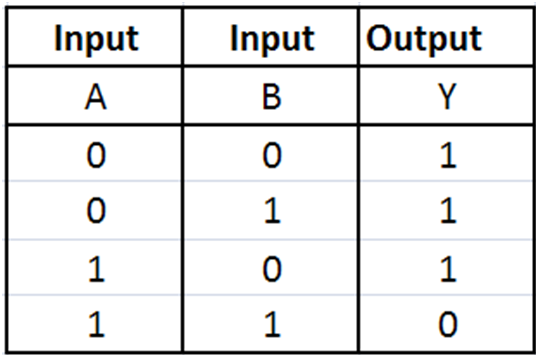
\includegraphics{img/exp4/2}
		\caption{Truth Table for NAND gate}
		\label{fig:4:2}
	\end{figure}
	
	A simple 2-input logic NAND gate can be constructed using RTL (Resistor-transistor-logic) switches connected together as shown below with the inputs connected directly to the transistor bases. Either transistor must be cut-off or “OFF” for an output at Q.
	
	\begin{figure}[h]
		\centering
		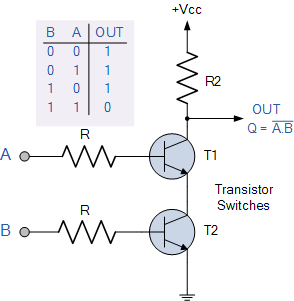
\includegraphics{img/exp4/3}
		\caption{Circut for making NAND gate}
		\label{fig:4:3}
	\end{figure}
				
\section{Procedure}
	\subsubsection{Simulator 1}
	\begin{itemize}
		\tightlist
		\item Connect the supply(+5V) to the circuit.
		\item Press the switches for inputs "A" and "B".
		\item The bulb glows if any one or both the switches are OFF else it won't glow.
		\item Repeat step-2 and step-3 for all state of inputs.
	\end{itemize}

	\subsubsection{Simulator 2}
	\begin{itemize}
		\tightlist
		\item Enter the Boolean input "A" and "B".
		\item Enter the Boolean output for your corresponding inputs.
		\item Click on "Check" Button to verify your output.
		\item Click "Print" if you want to get print out of Truth Table.
	\end{itemize}


\section{Observations}
	\begin{figure}[h]
		\centering
		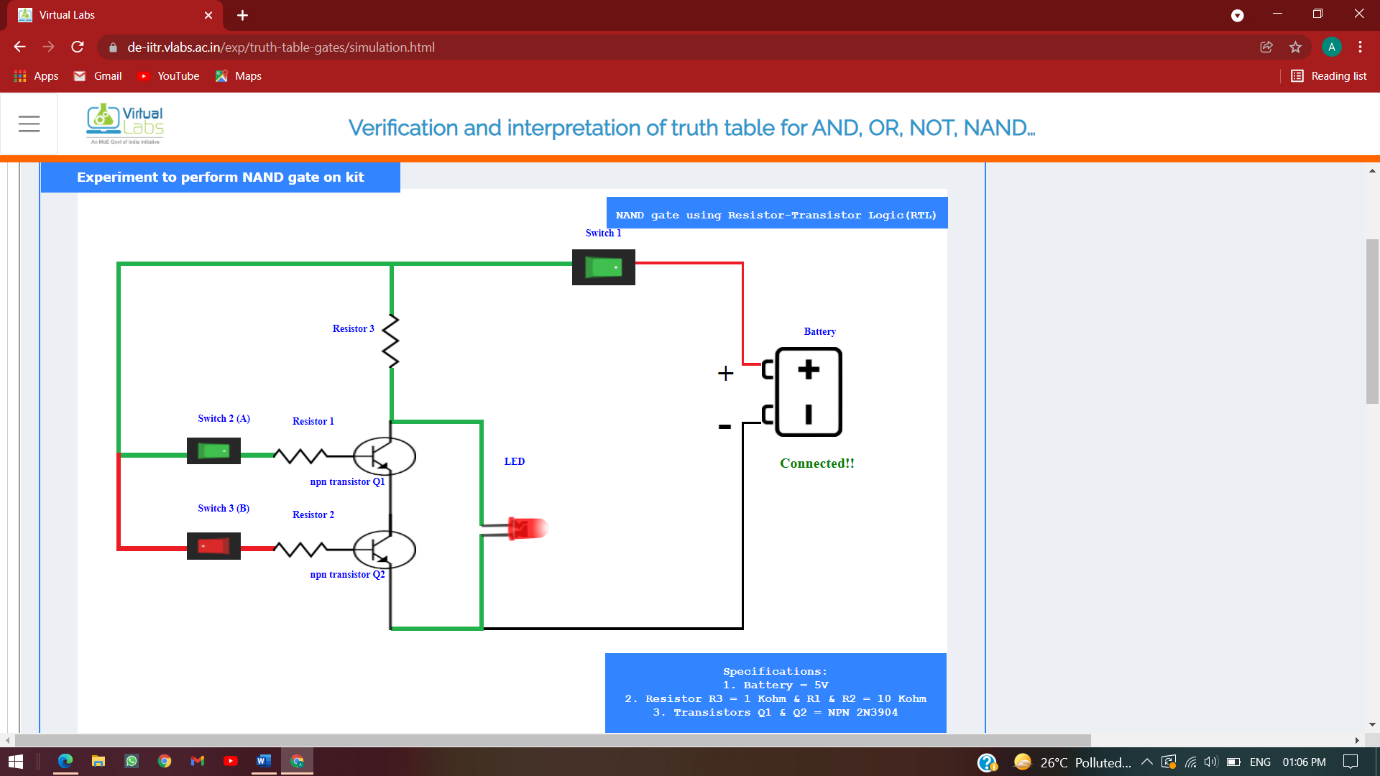
\includegraphics[width=0.9\linewidth]{img/exp4/4}
		\caption{}
		\label{fig:4:4}
	\end{figure}
		\begin{figure}[h]
		\centering
		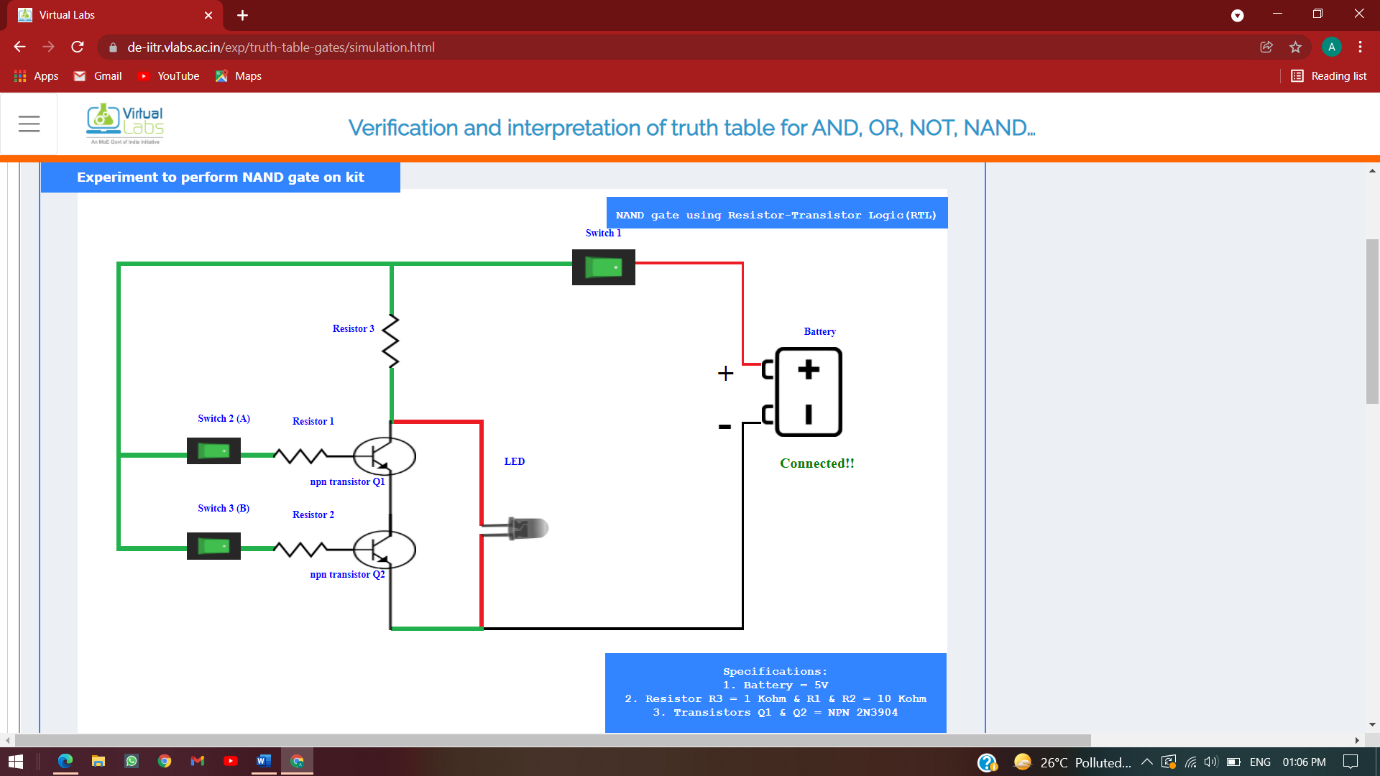
\includegraphics[width=0.9\linewidth]{img/exp4/5}
		\caption{}
		\label{fig:4:5}
	\end{figure}
		\begin{figure}[h]
		\centering
		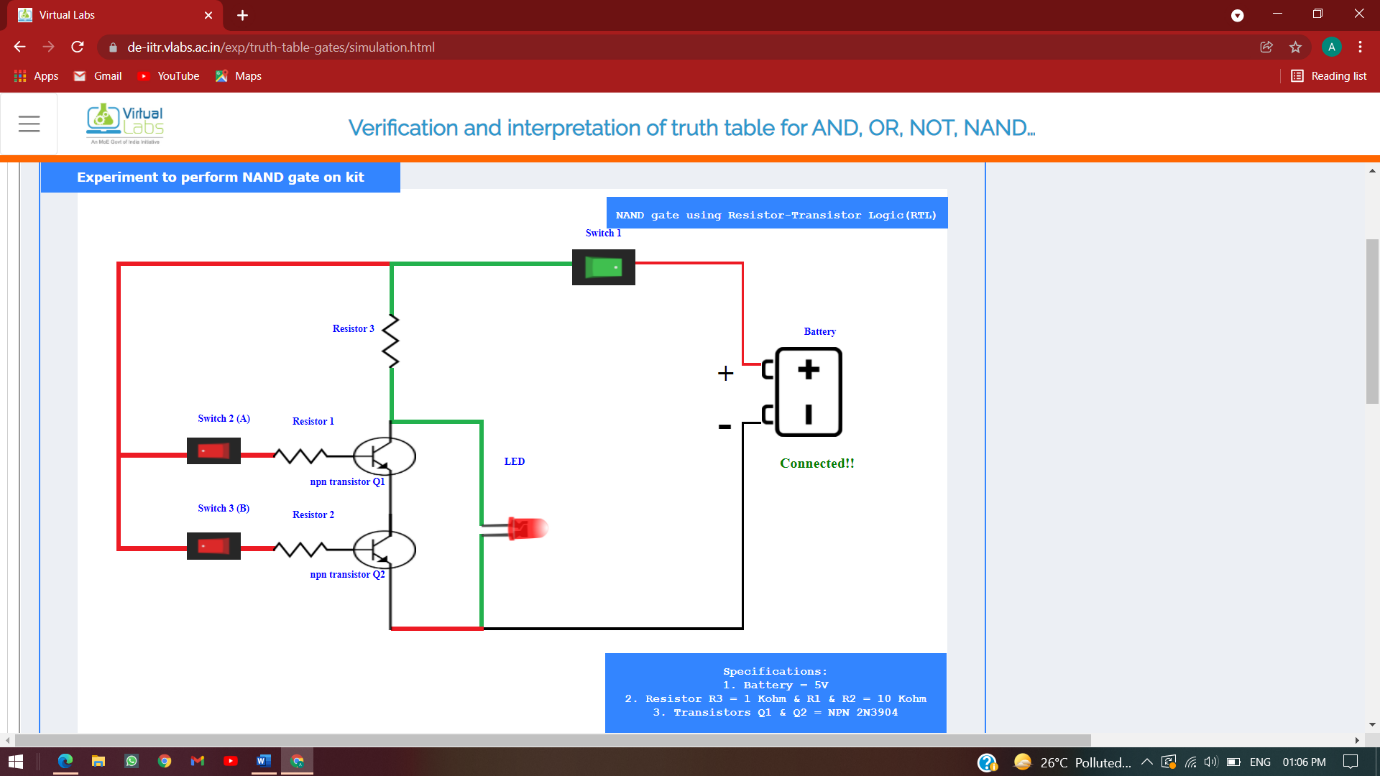
\includegraphics[width=0.9\linewidth]{img/exp4/6}
		\caption{}
		\label{fig:4:6}
	\end{figure}
		\begin{figure}[h]
		\centering
		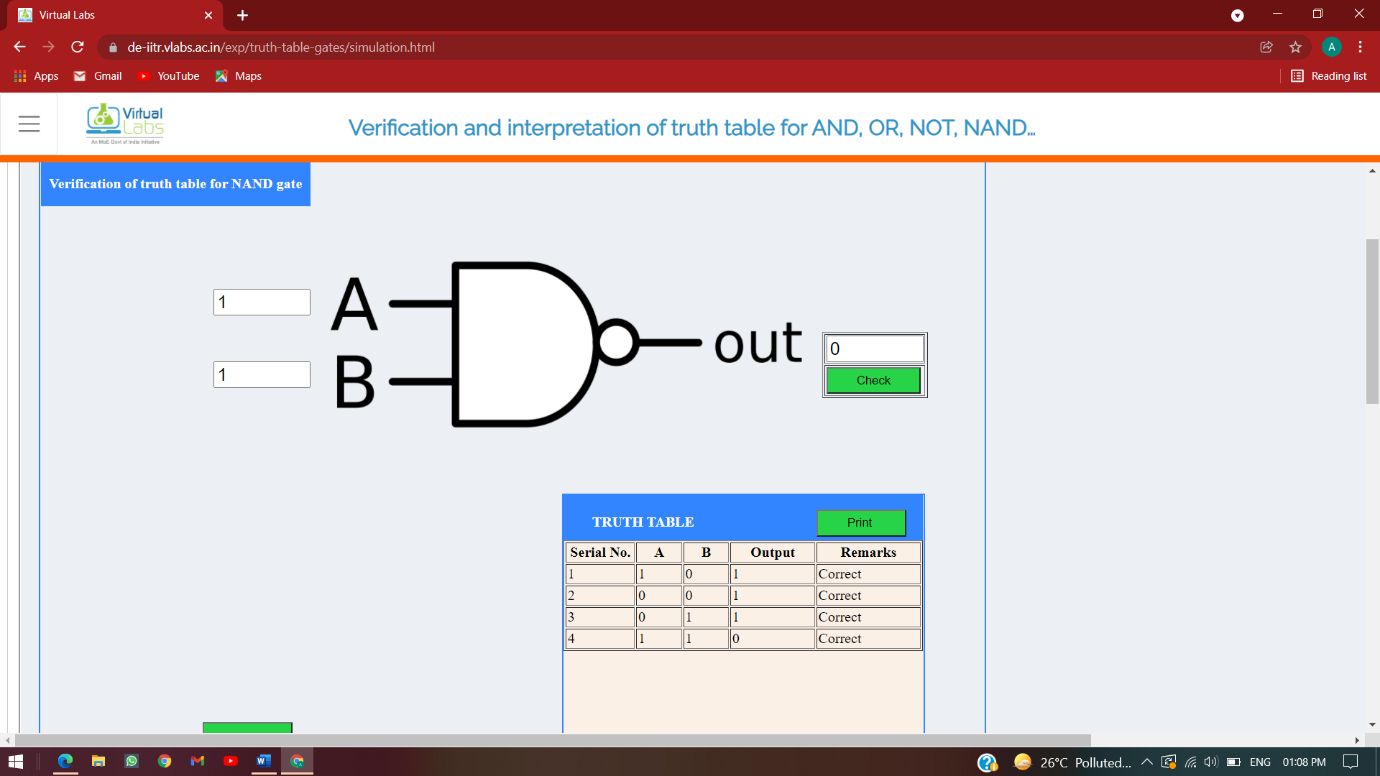
\includegraphics[width=0.9\linewidth]{img/exp4/7}
		\caption{}
		\label{fig:4:7}
	\end{figure}

\section{Conclusion}
NAND gate basically negates the results of AND gate . The output is low when both the inputs are high and the output is high when even one of the input is low.

\section{Precautions}
	\begin{enumerate}
		\tightlist
		\item Make the connections when power supply is OFF.
		\item Ensure that the connections are tight.
		\item Change the status of inputs only when power supply is OFF.
	\end{enumerate}